
\documentclass{mcmthesis}
\mcmsetup{CTeX = true,   % 使用 CTeX 套装时,设置为 true
        tcn = 0000, problem = A,
        sheet = true, titleinsheet = true, keywordsinsheet = true,
        titlepage = true, abstract = true}
\usepackage{newtxtext}%\usepackage{palatino}
\usepackage{lipsum}
\usepackage{subfigure}
\title{The \LaTeX{} Template for MCM Version \MCMversion}
\author{\small \href{https://www.latexstudio.net/}
  {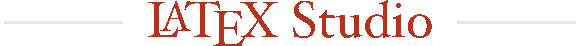
\includegraphics[width=7cm]{mcmthesis-logo}}}
\date{\today}
\begin{document}
\begin{abstract}
Use this template to begin typing the first page (summary page) of your electronic report. This template uses a 12-point Times New Roman font. Submit your paper as an Adobe PDF electronic file (e.g. 1111111.pdf), typed in English, with a readable font of at least 12-point type.

Do not include the name of your school, advisor, or team members on this or any page.

Papers must be within the 25 page limit.


Be sure to change the control number and problem choice above.
You may delete these instructions as you begin to type your report here.

Follow us @COMAPMath on Twitter or COMAPCHINAOFFICIAL on Weibo for the most up to date contest information.

\begin{keywords}
keyword1; keyword2
\end{keywords}
\end{abstract}
\maketitle
%% Generate the Table of Contents, if it's needed.
%% \tableofcontents
%% \newpage
%%
%% Generate the Memorandum, if it's needed.
%% \memoto{\LaTeX{}studio}
%% \memofrom{Liam Huang}
%% \memosubject{Happy \TeX{}ing!}
%% \memodate{\today}
%% \logo{\LARGE I'm pretending to be a LOGO!}
%% \begin{memo}[Memorandum]
%%   \lipsum[1-3]
%% \end{memo}
%%

\newpage
\thispagestyle{empty}
\tableofcontents
\newpage



\section{Introduction}
\subsection{Background}
随着个人资产的累计,越来越多的人进入投资市场,为了在使现有资产保值或更有价值。
但我们都知道,投资类产品常有很强的波动性,which means 它很难预测。
在众多投资产品中,黄金和比特币最受人关注。
特别是比特币,自出现以来交易规模迅速扩张,但巨大的价格波动使其安全性和稳定性受到质疑。
那么,在黄金和比特币投资热潮下,对普通交易者大幅度得利的投资组合很难实现。
这是很重要的,根据每天和前几天更新的交易数据,来预测未来波动性资产的发展趋势。
因此,交易者提出 to develop a model that uses only the past stream of daily prices 
to date to determine each day if the trader should buy, hold, or sell their assets in their portfolio.


\subsection{Problem Statement}


\subsection{Problem Analysis}
为了更好的帮助交易者做出每日投资决策,我们



\iffalse
\begin{itemize}
\item the angular velocity of the bat,
\item the velocity of the ball, and
\item the position of impact along the bat.
\end{itemize}

\begin{Theorem} \label{thm:latex}
\LaTeX
\end{Theorem}
\begin{Lemma} \label{thm:tex}
\TeX .
\end{Lemma}
\begin{proof}
The proof of theorem.
\end{proof}

\begin{itemize}
\item
\item
\item
\item
\end{itemize}
\fi                          %整段注释



\section{Assumption}



\section{Data Processing}
\subsection{Data Screening}

\subsection{Data Visualization}

\subsection{Mining Time Series}


%\begin{figure}[h]
%\small
%\centering
%\subfigure[1]{
%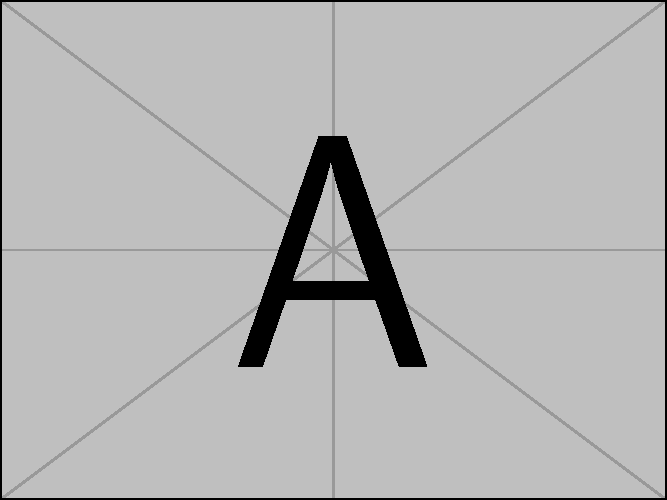
\includegraphics[width=0.3\columnwidth]{example-image-a}}
%\hfill
%\centering
%\subfigure[2]{
%  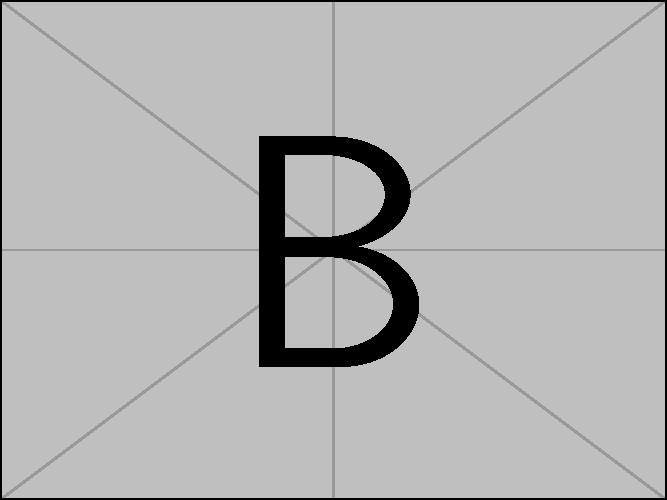
\includegraphics[width=0.3\columnwidth]{example-image-b}}
%\caption{The name of figure} \label{fig:aa}
%\end{figure}

%\lipsum[8] \eqref{aa}
%\begin{equation}
%a^2 \label{aa}
%\end{equation}
\iffalse
\[
  \begin{pmatrix}{*{20}c}
  {a_{11} } & {a_{12} } & {a_{13} }  \\
  {a_{21} } & {a_{22} } & {a_{23} }  \\
  {a_{31} } & {a_{32} } & {a_{33} }  \\
  \end{pmatrix}
  = \frac{{Opposite}}{{Hypotenuse}}\cos ^{ - 1} \theta \arcsin \theta
\]


\[
  p_{j}=\begin{cases} 0,&\text{if $j$ is odd}\\
  r!\,(-1)^{j/2},&\text{if $j$ is even}
  \end{cases}
\]


\[
  \arcsin \theta  =
  \mathop{{\int\!\!\!\!\!\int\!\!\!\!\!\int}\mkern-31.2mu
  \bigodot}\limits_\varphi
  {\mathop {\lim }\limits_{x \to \infty } \frac{{n!}}{{r!\left( {n - r}
  \right)!}}} 
\]
\fi



\section{PartⅠ:Model Development }
\subsection{Time Series Model ARIMA - Data Forecasting }
\subsubsection{Stability Test}%翻译

\subsubsection{White Noise Test}%翻译

\subsubsection{Train the Model With All the Data}

\subsubsection{Model Validating}

\subsubsection{Model Prediction and Visualization}

\subsubsection{Batch prediction of data }   %去未来七天


\subsection{Investment Decision Model - Dynamic Programming }
%流程图
\iffalse
\begin{figure}[!hb]
    \centering  %图片居中显示        %路径不能有中文
    \includegraphics[width=3cm]{jinyue.png}
    \caption{这是美丽喀纳斯} \label{kanasi}
 \end{figure}
\fi

\subsubsection{Buy and Sell Standard Setting}

\subsubsection{Portfolio Optimal Ratio Identification}

\subsubsection{Positioning Standard Identification}

\subsubsection{Daily Portfolio Determinations}






\section{PartⅡ:Strategy Evaluation}
\subsection{Set Perturbation Terms }%to determine optimal parameters }

\subsection{Comparison Illustrates the Best Strategy}




\section{PartⅢ:Sensitivity Analysis}
\subsection{Assuming Changes In Commission}

\subsection{Visualization Results}%Analysis ensitivity}





\section{Evaluate of the Model}
\subsection{Strengths and weaknesses}

\subsection{Sensitivity Analysis}




\section{Conclusions}


\section{A Memo}






\begin{itemize}
\item \textbf{Applies widely}\\
This  system can be used for many types of airplanes, and it also
solves the interference during  the procedure of the boarding
airplane,as described above we can get to the  optimization
boarding time.We also know that all the service is automate.
\item \textbf{Improve the quality of the airport service}\\
Balancing the cost of the cost and the benefit, it will bring in
more convenient  for airport and passengers.It also saves many
human resources for the airline. \item \textbf{}
\end{itemize}

\begin{thebibliography}{99}
\bibitem{1} D.~E. KNUTH   The \TeX{}book  the American
Mathematical Society and Addison-Wesley
Publishing Company , 1984-1986.
\bibitem{2}Lamport, Leslie,  \LaTeX{}: `` A Document Preparation System '',
Addison-Wesley Publishing Company, 1986.
\bibitem{3}\url{https://www.latexstudio.net/}
\end{thebibliography}

\begin{appendices}

\section{First appendix}

In addition, your report must include a letter to the Chief Financial Officer (CFO) of the Goodgrant Foundation, Mr. Alpha Chiang, that describes the optimal investment strategy, your modeling approach and major results, and a brief discussion of your proposed concept of a return-on-investment (ROI). This letter should be no more than two pages in length.







\begin{letter}{Dear, Mr. Alpha Chiang}

\vspace{\parskip}

Sincerely yours,

Your friends

\end{letter}
Here are simulation programmes we used in our model as follow.\\

\textbf{\textcolor[rgb]{0.98,0.00,0.00}{Input matlab source:}}
\lstinputlisting[language=Matlab]{./code/mcmthesis-matlab1.m}

\section{Second appendix}

some more text \textcolor[rgb]{0.98,0.00,0.00}{\textbf{Input C++ source:}}
\lstinputlisting[language=C++]{./code/mcmthesis-sudoku.cpp}

\end{appendices}
\end{document}
%% 
%% This work consists of these files mcmthesis.dtx,
%%                                   figures/ and
%%                                   code/,
%% and the derived files             mcmthesis.cls,
%%                                   mcmthesis-demo.tex,
%%                                   README,
%%                                   LICENSE,
%%                                   mcmthesis.pdf and
%%                                   mcmthesis-demo.pdf.
%%
%% End of file `mcmthesis-demo.tex'.